\documentclass{bmvc2k}

%% Enter your paper number here for the review copyu
\bmvcreviewcopy{666}

\title{Correspondence matching of non-coplanar circles from a single image}

% Enter the paper's authors in order
% \addauthor{Name}{email/homepage}{INSTITUTION_CODE}
\addauthor{Susan Student}{http://www.vision.inst.ac.uk/~ss}{1}
\addauthor{Petra Prof}{http://www.vision.inst.ac.uk/~pp}{1}
\addauthor{Colin Collaborator}{colin@collaborators.com}{2}

% Enter the institutions
% \addinstitution{Name\\Address}
\addinstitution{
 The Vision Institute\\
 University of Borsetshire\\
 Wimbleham, UK
}
\addinstitution{
 Collaborators, Inc.\\
 123 Park Avenue,\\
 New York, USA
}

\runninghead{Student, Prof, Collaborator}{BMVC Author Guidelines}

% Any macro definitions you would like to include
% These are not defined in the style file, because they don't begin
% with \bmva, so they might conflict with the user's own macros.
% The \bmvaOneDot macro adds a full stop unless there is one in the
% text already.
\def\eg{\emph{e.g}\bmvaOneDot}
\def\Eg{\emph{E.g}\bmvaOneDot}
\def\etal{\emph{et al}\bmvaOneDot}

%------------------------------------------------------------------------- 
% Document starts here
\begin{document}

\maketitle

\begin{abstract}
In this work we have proposed a method to determine 2D-3D correspondence between non-coplanar circles from a single image.
Our method uses image conics to compute circle plane orientation in camera coordinate system, thus bringing the problem from 2D to 3D domain. This information is used to generate projective invariant descriptors which can be used directly for correspondence matching, given that the 3D information about circles are known. Additionally, the evaluation also covers study stability of the projective invariants and the factors affecting their computation. One of the intended applications is for tracking industrial objects with circles on it. In our approach we use conic properties of circles to compute projective invariant descriptors. These descriptors are matched with known 3D information to establish correspondences. We also demonstrate stability of the invariants used to generate descriptors both in practice and simulation. 
In our approach we compute 3D plane orientation of each circle from its image contour, and compute projective invariants between each pair of circles. We propose a new descriptor 

\end{abstract}

%------------------------------------------------------------------------- 
\section{Introduction}
\label{sec:intro}
goal : 
Explain the problem in question, the motivation for the work and the proposed application in mind. The assumptions made in our work. We have the camera calibrated and we use 3D points and their normal positions for the descriptor measurement. 
%No much work done in this direction. The invariants proposed are never used for a application so we provide use and discuss stability of the algorithm. Comment on why circles and the paper we build up to. 
%The work of Forsyth as the base of our work, the concepts given in the paper. Our contribution is matching strategy using such invariants. Demonstrating an application and evaluation of the method. 

Correspondence matching is one of the key problems in computer vision. Applications related to pose estimation or object detection require accurate knowledge of model features and their corresponding image features. 
The problem becomes more challenging for monocular systems as the depth information is lost. Popular monocular methods involve learning object with few initial frames or require initialisation to facilitate matching [N3M so on]. Many authors have proposed using natural features like points, lines and conics for solving correspondence problem \cite{hartley_multiple_2003}. Such features are easier to extract from images and can be used to compute reliable projective invariants. Invariants are extensively studied topic in early vision community, Forsyth \etal \cite{forsyth_91} provided a detailed account on 3D invariant descriptors and their stability under projective motion. 
In learning based model tracking methods initial frames of the camera are used to learn model and compute unique descriptors from dense or sparse set of natural model features \cite{chekhlov_ninja_2007} \cite{hinterstoisser_n3m:_2007} \cite{lowe_object_1999}. Other methods involve using a selective set features (edges, contours, etc.) to compute invariants from a single image \cite{lepetit_monocular_2005}. In our method we demonstrate how non-planar circular features can be used to compute invariant descriptors and solve matching from single image. 
%We propose one such method for multiple non-coplanar circular features exist in the scene. solving correspondence problem when 
%Machine learning based methods \cite{Hartley00} provide promising results, but are limited to a specific group of objects and require prior learning of the object. 
%This work is focussed on finding correspondence information from a single image of the scene. 
%Methods [quan] find correspondence    

%Many authors have proposed using natural features like points, lines and conics for solving correspondence problem. 
%The core idea is to compute projective invariants from such features to obtain robust matching with model feature points.
%[Quan] One approach is using two or more images from different perspective to find same image features and then obtain correspondence using triangulation technique. 
%The problem is more complex with a single image as depth feature is lost. 
%In this paper we will focus on solving this particular problem of matching from a single image. 

In single images projective transformation of features make it difficult to compute invariant features. Coplanar conics, lines and points can be used to compute planar invariants \cite{forsyth_91}. Circles have a special property to retain depth information under projective transformation. A world circle always produces an elliptical curve on the image plane. If size of circle is known orientation of circle plane can be defined in 3D (camera coordinates) with a two fold ambiguity \cite{forsyth_91} \cite{safaee-rad_three-dimensional_1992}. 
Further, Forsyth \etal \cite{forsyth_91} proposed that up to three projective invariant can be computed from a non-coplanar pair of circles. They explain that angle between circle planes (angle between surface normals) and distance between centre of the circles are invariant quantities. The concept was proposed in early 90s, however these invariants have remained unexplored. 
We propose using these invariants to solve correspondence problem when multiple 3D circular features exist on a model. 
In this approach we bring problem from 2D to 3D by computing 3D invariants from image features, then solve 3D-3D matching problem with model. (Fig of decsriptor match) 
We use invariant descriptors (computed from elliptical image features) to solve the conic ambiguity and provide accurate matching with 3D features. 
The proposed method is first attempt to use these invariants, therefore we also carried out simulations to show stability of invariants against change of perspective.  

%We demonstrate  practical scenario where such method can be used effectively.
Our contribution is a new method to accurately identify image correspondences when multiple identical 3D circular features exist in the scene. We assume that calibration of camera is known and 3D information of features is available. 
Often in Industry based model tracking applications 3D-CAD data is known. Our matching method is suitable for tracking any 3D objects having known circles on different planes. In close range photogrammetry multiple circular markers (fig) are placed on 3D models for surface measurements \cite{luhmann_close_2006}. 
These measurements include computation of surface normal and 3D position of each marker. 
This process involves taking multiple images of the model with additional presence of encoded markers in the scene to solve correspondence. 
Once 3D measurements are done our method can be extremely useful to support tracking application without using coded patterns. Similarly various industrial parts having natural circles can be identified and tracked with this method. 
We prepared two car models with circular markers for evaluating our matching method. The proposed method can find corresponding circular marker from a single image, with high accuracy. We also show that our method is stable against false positives detected from the scene. Our method is fast enough to support real-time tracking applications. 

[REFER : Comment on descriptor being propose of 3D point an normal based info. ]

%-> Figure explaining the issue 
%\begin{figure}
%\begin{tabular}{ccc}
%\bmvaHangBox{\fbox{\parbox{2.7cm}{~\\[2.8mm]
%\rule{0pt}{1ex}\hspace{2.24mm}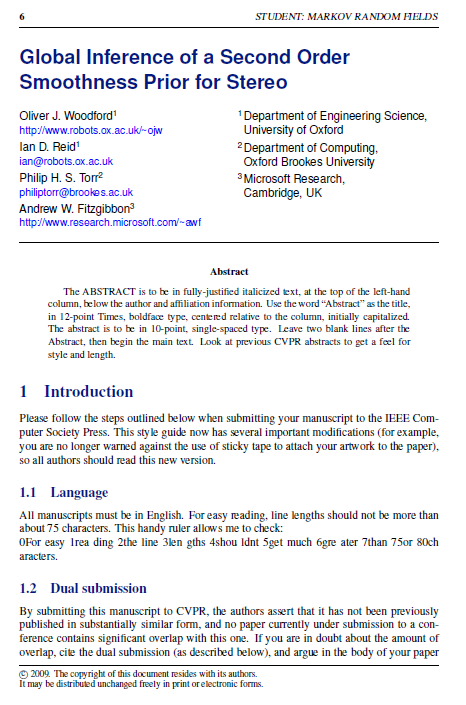
\includegraphics[width=2.33cm]{images/eg1_largeprint.png}\\[-0.1pt]}}}&
%\bmvaHangBox{\fbox{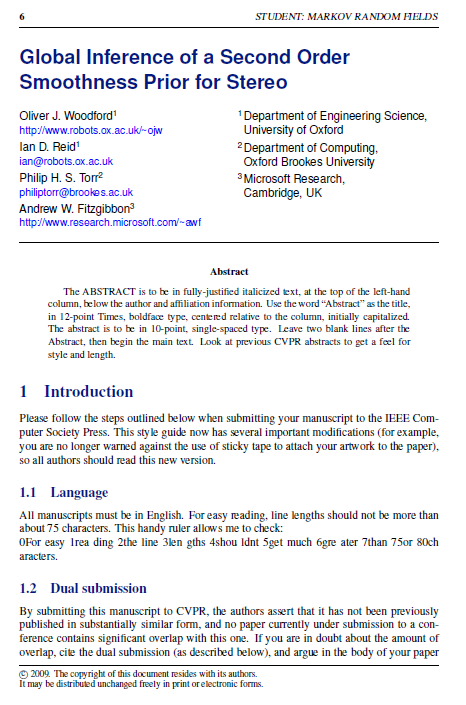
\includegraphics[width=2.8cm]{images/eg1_largeprint.png}}}&
%\bmvaHangBox{\fbox{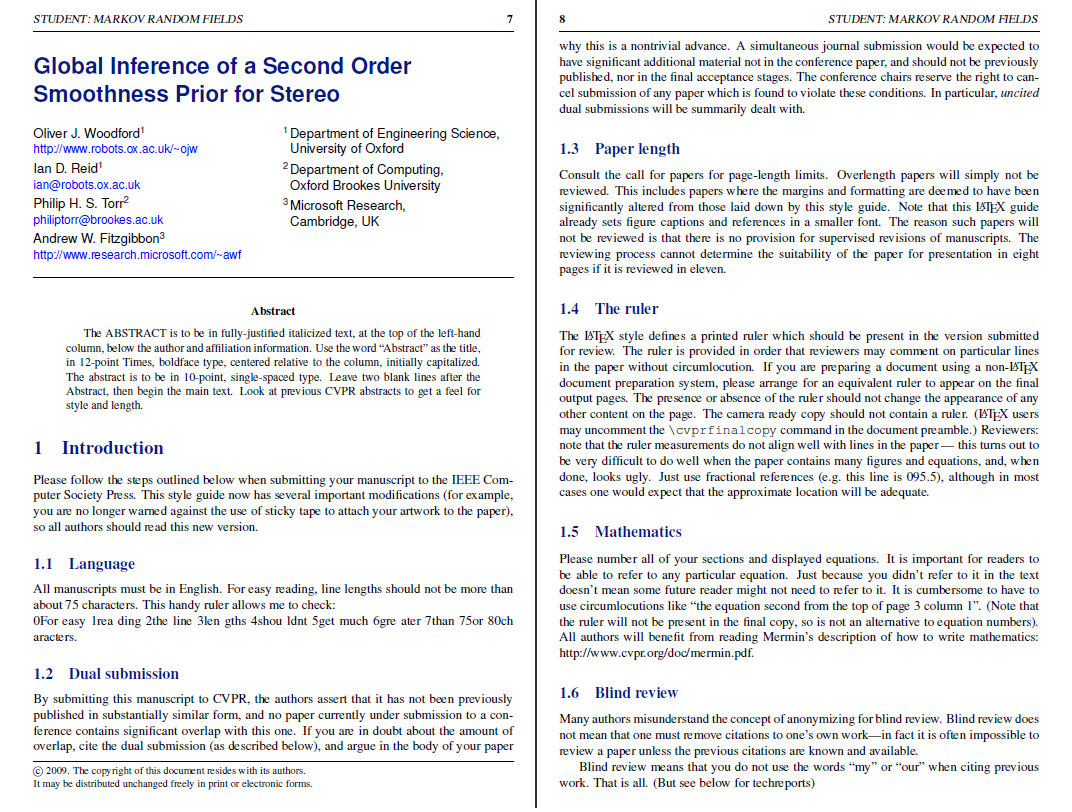
\includegraphics[width=5.6cm]{images/eg1_2up.png}}}\\
%(a)&(b)&(c)
%\end{tabular}
%\caption{It is often a good idea for the first figure to attempt to
%encapsulate the article, complementing the abstract.  This figure illustrates
%the various print and on-screen layouts for which this paper format has
%been optimized: (a) traditional BMVC print format; (b) on-screen
%single-column format, or large-print paper; (c) full-screen two column, or
%2-up printing. }
%\label{fig:teaser}
%\end{figure}

\section{Related Work}

Object detection and pose estimation from conic features is widely studied in 3D vision literature  \cite{dhome_spatial_1990}\cite{safaee-rad_three-dimensional_1992} \cite{werghi_pose_1996} \cite{quan_invariant_1995}. Circular shape is also a popular choice for designing artificial fiducial. Detection of contour points from image and fitting ellipse is a well studied topic \cite{fitzgibbon_direct_1999}. 
%Detection of conic sections from the image is easy and also a widely studied subject [conic fitting, gibbon].
Quan \cite{quan_conic_1996} proposed a two view approach for finding correspondence and 3D reconstruction with conic section. Authors have proposed methods to compute invariants for coplanar conics \cite{forsyth_91} \cite{Ferri_1993}.  
%Various tracking and camera calibration methods use a pair coplanar circular features to compute invariant descriptors. 
A 3D problem is simplified to 2D when coplanar features are recovered and used for correspondence.  
Ying \etal \cite{ying_camera_2007} use a coplanar pair for camera calibration. 
Uchimaya \etal \cite{uchiyama_random_2011} developed invariant descriptors from multiple coplanar circles, and extended the work for deformable model \cite{uchiyama_deformable_2011}.
\cite{lo_pez_de_ipin_a_trip:_2002} \cite{naimark_circular_2002} \cite{pagani_circular_2011} propose a circular marker for 6D pose estimation, no invariants are computed as correspondence is solved by using unique coded pattern around the circle. 
\cite{lo_pez_de_ipin_a_trip:_2002}\cite{pagani_circular_2011} use circular shape to define circle plane in 3D, Additionally use a coded pattern is used encode 6D pose without ambiguity.(Fig). 
Luhmann \cite{luhmann_close_2006} provides detailed account of methods using point circular fiducials in close range Photogrammetry. The current state of the art methods coded patterns are introduced to simplify correspondence problem.
[GOM][AICON] are one of the industrial supplies for close range photogrammetry measurement equipments. 

[Refer Thesis: Comment on catalogue based methods, ]
\paragraph{}
Literature study suggests that, existing methods either provide a solution for coplanar circular features or non-coplanar  coded circular features. The novelty of our method is that it addresses 2D-3D matching problem for non planar circles present in the scene. 

\section{Method}
We assume that both 2D and 3D data is already available, and will focus on the matching method in detail. 
3D data includes the surface normal ($N_i$), centre position ($M_i$) and size ($R_i$) of the circles on the model. 
2D data includes centre points ($m_i$) and conic matrices ($C_i$) recovered from the undistorted image. The camera intrinsics ($K$) and distortion parameters are known. We have followed approach of Naimark \cite{naimark_circular_2002} and Fitzgibbon \cite{fitzgibbon_direct_1999} for ellipse detection and fitting.  

\subsection{Invariants}
%The invariants generate by a pair of non-planar circles is explained by Forsyth \etal \cite{forsyth_91}. 
If camera's projection centre is assumed as the vertex of a cone which has the world circle is at its base.
The image plane can be considered as a cutting plane $\pi$, which always creates an elliptical cross section.  
%Theory of conic sections can be used to suggest that the image projections are nothing but a cross section of a cone. 
A new plane $ \pi' = T* \pi $ can be computed such that intersection of plane $\pi'$ with the cone is circular. 
%A rotation transformation $T$ can be applied to the image plane such that the intersection of transformed plane $\pi'$ with the cone is a perfect circle. 
Plane ($\pi'$) is parallel to the base of the cone hence a plane normal $Nc_i$ can be computed from $T$. 
Additionally, 3D position of circle centre $Mc_i$ can be computed in camera coordinate system if original radius is known.
A normal $Nc_i$ and a point on plane $Mc_i$ are sufficient to define the plane of circle in camera coordinate system.
$ T $ is a combination of two rotations \cite{forsyth_91}\cite{lo_pez_de_ipin_a_trip:_2002}, one of the two has $\pm \phi$ rotation angle which introduces the ambiguity (two solutions) in plane recovery. 
This implies that every image conic results in to two possible plane orientations, we call this method as Ellipse Backprojection. 
\begin{equation}
\text{Ellipse Backprojection}(m_i,C_i) \rightarrow {Nc_i}^1,{Nc_i}^2,{Mc_i}^1,{Mc_i}^2
\end{equation}
Forsyth \etal \cite{forsyth_91} explained that for three dimensional objects descriptors consist of euclidean invariants rather than projective invariants. We use following invariants for our method, 
\begin{enumerate}
	\item \textbf{Angle between planes} ($\theta$) : It is same as angle between their surface normals 
	(i.e. $ \angle(Nc_i,Nc_j) $). $\theta$ can be recovered from conic image without knowledge of circle size in real world.  
%	\item \textbf{Ratio of circle radius to distance between circle centers}: This invariant can also be recovered without radius value.
	\item \textbf{Distance between circle centres} : This vector $ V $($ Mc_i,Mc_j $) has three degrees of freedom. The length of the vector $d_c$ is invariant (object scale should be known) and consistent despite of the ambiguity. 
\end{enumerate}
It should be noted that ambiguity of Ellipse Backprojection produces 4 solutions for $\theta$, only one of which is correct. 
Other invariants can be computed from recovered normal and centre values. These invariants are unstable \cite{forsyth_91} as the error from both recovered components influences the computation.
The quality of Ellipse Backprojection depends on distance from the camera and the viewing angle (angle between the image plane and the circle plane)\cite{werghi_pose_1996}. 
We performed simulations for circles of diameter ($\phi$) of 5,8,12 mm to understand behaviour of Ellipse Backprojection on small features. We varied the camera distance (0.5 to 2 m) and viewing angle (0-70$^\circ$) in step wise manner, while recording 100 iterations at each step.
At low viewing angles 0-10$^\circ$ both angle and centre recovery has higher errors, at any fixed distance. 
The shape of ellipse is almost circular at small viewing angles, this factor can explain high errors. 
Error in estimation grows with camera distance, however normal recovery appears less sensitive to camera distance than centre recovery. The comparison of the ambiguity explains that estimated centres ($ {Mc_i}^1,{Mc_i}^2 $) are very close to each other ($\leq$ 0.1 mm for $\phi$=12 mm), therefore any one of the solutions can be chosen. We can conclude that normal recovery has less errors but computation of $\theta$ will result in 4 solutions. The centre recovery is prone to errors, however has a unique solution (all 4 solutions are consistent).

\subsection{Descriptor design}
After ellipse back projection method 
The observations from simulations suggest that for a pair of image conics we obtain following information, 
\[ 
C_i,C_j \rightarrow d_c,\theta_{11},\theta_{12},\theta_{21},\theta_{22}
\]
where $\theta_{ij} = \angle ({Nc_i}^i)$


The simulations done for the invariants are commented and comments are made on 
A descriptor represents two unique points and not one point. Unlike many methods used these days. 
<d,theta>, <d,th1,th12,th21,th22>. 
Since both are not exactly same a matching strategy is developed to have point to point correspondence.    
\subsection{Step 1: Initial Pairwise Matching}
- Algorithm (Select pairs as tentitive matches by matching d and theta with some threshold)
- Explain the pairwise matching 
%------------------------------------------------------------------------- 
\subsection{Step 2: Triplet Matching}
Why? : because of ambiguity lot of results are false, by adding another constraint we restrict the probability of false matching. Also to make it point wise problem from a pair wise problem. 
- Matching steps on voting 
- Solving problem from pairwise matching to point wise matching
\subsection{Step 3: Hypothesis generation}
Filter the voting matrix to generate point wise matching hypothesis. 
Comment on how many would be enough to check other hypothesis. 
(3 are enough to predict solutions) since we know the calibration. 
One can select only top voted 3 pairs (since they are 3D points) and then verify the whole choice, or go for 6 point matching and achieve the same.

%\begin{figure*}
%\begin{center}
%\fbox{\rule{0pt}{2in} \rule{.9\linewidth}{0pt}}
%\end{center}
%   \caption{Example of a short caption, which should be centered.}
%\label{fig:short}
%\end{figure*}

%\begin{table}
%\begin{center}
%\begin{tabular}{|l|c|}
%\hline
%Method & Frobnability \\
%\hline\hline
%Theirs & Frumpy \\
%Yours & Frobbly \\
%Ours & Makes one's heart Frob\\
%\hline
%\end{tabular}
%\end{center}
%\caption{Results.   Ours is better.}
%\end{table}

\section{Evaluation}
Page 5: 
Explain the experiment model preparation. The selection of the markers as per standard. Good detection range with such sizes to give reader idea of tracking range. 
Model 1 : 12mm 
Model 2 : 8mm-5mm 
Ground truth : GOM data for 3D information and ground truth for 3D and 2D correspondences. 

Descriptor matching success prediction: Synthetic experiments that mimic real world moving planes, with small and big markers to understand the expected outcome. With the given choice of thresholds for descriptor matching. 

%------------------------------------------------------------------------- 
\subsection{Matching comparison}
%1. Exp 1 : Models in the frame with different pose 
%Comment : How are images taken, Fixed camera distances 
%Table : No of input points , No of Matched points , No of correct Match, No of Images
%1. For model 12 mm : 75 Images 
%
%2. For model 5 mm : 75 Images (8 mm markers covered)
%
%3. For model 8 mm : 75 Images (5 mm markers covered)
%
%
%2. Exp 2 : Models in presence of each other (False positive rejection (on and off the model) )
%Images taken with all models in the scene, the exact images are used to track all 3 models  
%1. 12mm car with 8mm/5mm car model 
%
%2. 8 mm with 5mm on itself (Bad results) : Is this experiment important? or Experiment with other model with 12 mm configuration. (Bad matching results removed by voting filtering). 
%
%3. 12 mm with 130 false positives and computing the right model. 
%------------------------------------------------------------------------
%\subsection{Time}
%Time taken for high resolution images and low resolution images. Tracking applications specific performance comments. Suitable for real time applications like in AR. 
%
%Time analysis from thesis : 
%- 2-3 FPS support to 5 Megapixel (0.35\% of tracking time)
%- 7-8 FPS support to web cam (1.34 \% of tracking time)
%
%- 100+ False positives make time as less as 50 \% of tracking time. 

\section{Conclusion}
Page 7 : 
1. Reliable method for correspondence matching for non coplananr circular features. 
2. Accuracy is improved with the size and method works better if the detection range is selected appropriate to the conic size. 
3. Comment on the stability of the invariants 
4. Comment on arrangement of the circles. (Random and non symmetric)


\section{Future Applications}
Future work : 
1. 2D-2D correspondence to triangulate from multiple images to get rid of the initial condition. 
2. Improving the matching method for higher runtime performance.
3. Using normals obtained for solving p3p problem. 

Each model has its own orientation and random arrangement gives us choice between tracking same models with individual identity. 


\bibliography{egbib}
\end{document}
